\chapter{线性空间}
\section{线性空间}
\begin{definition}{线性空间}{linear space}
	定义域$\FF$上的线性空间(linear space)~$V$是具有加法$+:V\times V\to V$和数乘$\cdot:\FF\times V\to V$运算且满足以下公理的集合。
	\begin{compactenum}
		\item 加法交换律\qqqquad\quad~$x+y=y+x;$
		\item 加法结合律\qqqquad\quad~$x+(y+z)=(x+y)+z;$
		\item 加法零元\qqqquad\qquad~$x+0=x;$
		\item 加法逆元\qqqquad\qquad~$x+(-x)=0;$
		\item 数乘单位元\qqqquad\quad~$1x=x;$
		\item 数乘结合律\qqqquad\quad~$(c_1c_2)x=c_1(c_2x);$
		\item 数乘对向量的分配律\quad$c(x+y)=cx+cy;$
		\item 数乘对标量的分配律\quad$(c_1+c_2)x=c_1x+c_2x.$
	\end{compactenum}
\end{definition}

\begin{example}
	{}{}
	$\FF^n$和$\FF^{m\times n}$都是线性空间。
\end{example}

\begin{definition}{子空间}{subspace}
	给定线性空间$V$的子集$V_\mathrm s\subset V$,若其对于加法和数乘封闭:$\forall v,w\in V_\mathrm s,\forall c\in\FF$
	\[
		v+w\in V_\mathrm s,\quad cv\in V_\mathrm s,
	\]
	则$V_\mathrm s$为$V$的子空间(subspace)。子空间中元素的线性组合都在同一个子空间,
\end{definition}

\begin{corollary}
	子空间必然包含零向量。因为若$v\in V_\mathrm s$,则$v+(-v)=0\in V_\mathrm s$。
\end{corollary}

\begin{remark}
	线性空间$V$的一个子集一般不是子空间,但我们可以通过其构造出子空间。
\end{remark}

\begin{definition}{线性扩张}{linear span}
	$S$的线性扩张(linear span)是$S$中向量的所有线性组合的集合,记作$\lspan(S)$。
\end{definition}

\begin{corollary}
	$V$的子集的线性扩展是$V$的子空间。
\end{corollary}

\section{线性独立、基和维度}
\begin{definition}{线性独立}{linear independent}
	$n$个向量$\{v_i\}$是线性独立的(linear independent),当且仅当
	\[
		\sum_{i=1}^nx_iv_i=0,
	\]
	只在$x_i=0$时成立,即只有零解。$n$个向量$\{v_i\}$不是线性独立,那么他们是线性相关的(linear correlate)。
	
	等价描述:集合中每一个向量都不能写成其它向量的线性组合。
\end{definition}
\begin{remark}
	向量是否线性独立同数域的选择有关。
\end{remark}
\begin{definition}{线性空间的基}{base}
	线性空间$V$的基(base)是一组线性无关的向量$\{v_i\}$,并且他们张成整个线性空间$V$。
\end{definition}
\begin{example}
	{}{}
	$\{e_1,\ldots,e_n\}$构成$\RR^n$的一组基。
\end{example}
\begin{definition}{线性空间的维度}{dimension}
	线性空间的维度(dimension)是一组基中向量的个数,记作$\dim(V)$。
\end{definition}
\begin{theorem}{维度的确定性}{certainty of dimension}
	线性空间的维度和基的选取无关。
\end{theorem}
\begin{proof}
	若线性空间$V$存在两组基$\{v_1,\ldots,v_m\},\{w_1,\ldots,w_n\}$元素个数不等,不妨设$n>m$。
	因为$\{w_i\}$是基,$\{v_i\}$可以被表示为其线性组合
	\[
		v_i=\sum_{j=1}^nw_ja_{ji},\quad\forall i.
	\]
	考虑线性组合
	\[
		\sum_{i=1}^mx_iv_i=\sum_{i=1}^m\sum_{j=1}^nx_iw_ja_{ji}=0.
	\]
	因为$\{w_i\}$线性无关,故
	\[
		\sum_{i=1}^ma_{ji}x_i=0,\quad\forall j,
	\]
	但是其未知数的个数$m>$方程的个数$n$,系数矩阵$A$一定有自由列,所以$x$有非零解。这与$\{v_i\}$线性无关矛盾!故$m=n.$
\end{proof}

\begin{theorem}{}{}
	若$\forall v\in V_1$可以写成$V_2$中向量的线性组合,则$\dim(V_1)\leqslant\dim(V_2)$。
\end{theorem}

\begin{proof}
	这个定理是trivial的,证明留给读者。
\end{proof}

\begin{definition}{变换矩阵}{transfomation matrix}
	不同基之间的变换相应的矩阵称为变换矩阵(transfomation matrix)。
\end{definition}

\section{矩阵\textit{A}的四个子空间}

给定矩阵$A\in\FF^{m\times n}$,可由其得到四个子空间:列空间、行空间、零空间和左零空间。
\begin{definition}{列空间和行空间}{column space}
	矩阵$A$的列空间(column space)是$A$的所有列的线性组合的集合,记作$\C(A)$:
	\begin{equation}
		\C(A)\equiv\set{Ax}{x\in\FF^n}.
	\end{equation}
	\tcblower
	矩阵$A$的行空间(row space)是$A$的所有行的线性组合的集合,%由于转置并不影响性质,行空间
	可用$\C(A\tp)$表示。
\end{definition}

\begin{corollary}
	$\C(A)$是$\FF^m$的子空间,$\C(A\tp)$是$\FF^n$的子空间。
\end{corollary}

\begin{remark}
	线性方程组$Ax=b$有解$\iff b\in\C(A)$。
\end{remark}

\begin{definition}{零空间和左零空间}{null space}
	矩阵$A$的零空间(null space)是所有满足$Ax=0$的$x$的集合,记作$\N(A)$:
	\begin{equation}
		\N(A)\equiv\set x{Ax=0}.
	\end{equation}
	\tcblower
	矩阵$A$的左零空间(left null space)是所有满足$x\tp A=0$的$x$的集合,可用$\N(A\tp)$表示。
\end{definition}

\begin{corollary}
	$\N(A)$是$\FF^n$的子空间,$\N(A\tp)$是$\FF^m$的子空间。
\end{corollary}

\begin{example}{子空间的基}{}
	$\N(A)$的基:显然$\N(A)=\N(\rref(A))$,而$\rref(A)$的每个自由列各给出一个$\N(\rref(A))$的基。若第$j$列为自由列,则其对应的基$x$的分量为:
	\[
		x_i=\begin{cases}
			\delta_{ij},&\text{第$i$列为自由列}\\
			-\rref(A)_{ij},&\text{第$i$列为主列}
		\end{cases}
	\]
	%$\dim(\rref(A))=\rref(A)$中自由列的数量;
	\tcblower
	$\C(A)$的基:$\rref(A)$的所有主列构成$\C(A)$的一组基。
\end{example}
\section{矩阵的秩、线性代数基本定理}
\begin{definition}{矩阵的秩}{rank}
	矩阵$A$的秩(rank)定义为列空间的维数:%\footnote{后面很快会证明行空间列空间维数相等。}:
	\[
		\rank(A):=\dim(\C(A)).
	\]
	若矩阵的秩等于行数,则称其行满秩(full row rank);
	若秩等于列数,则称其列满秩(full column rank)。
\end{definition}
\begin{theorem}
	{线性方程组$Ax=0$的完整解}{}
	线性方程组$Ax=b$的通解可以分解为特解$x_{\mathrm p}$和零解$x_{\mathrm n}$的和:
	\[
		x=x_{\mathrm p}+x_{\mathrm n},
	\]
	%其中$x_{\mathrm n}\in\N(A)$,
	特解满足$Ax_{\mathrm p}=b$,其各个分量可以由约化的增广矩阵$[\rref(A)\enspace b']$得到:
	\[
		(x_{\mathrm p})_i=\begin{cases}
			0,&\text{第$i$列为自由列}\\
			b'_j,&\text{第$i$列为主列,其主元1在第$j$行}
		\end{cases}
	\]
	而零解满足$Ax_{\mathrm n}=0$,可以写成零空间的基的线性组合。
\end{theorem}
\begin{corollary}
	~
	\begin{itemize}
		\item 若$A$列满秩,则$\rref(A)$没有自由列,$\N(A)=\{0\}$。当$b\in\C(A)$时有唯一解,否则无解;
		\item 若$A$行满秩,则$\rref(A)$没有零行,$\C(A)=\FF^m$,$\forall b$都有解,有唯一解或无穷多解。
	\end{itemize}
\end{corollary}
\paragraph{四个子空间的维度}已经知道,初等行变换就是用初等矩阵$E$左乘$A$,相应的,列变换就是$E$右乘$A$。
\begin{theorem}{初等变换和子空间}{}
	\begin{compactitem}
		\item $\N(A)=\N(EA)$,因为
		\[
			Ax=0\iff EAx=0.
		\]
		\item $\dim(\C(A))=\dim(\C(EA))$,因为
		\[
			\{v_i\}\text{~是~}\C(A)\text{~一组基}\iff\{Ev_i\}\text{~是~}\C(EA)\text{~一组基}.
		\]
		\item $\C(A)=\C(AE)$,因为
		\[
			AE\text{~的每一列}\in\C(A)\text{~且~}A=(AE)E\iv\text{~的每一列}\in\C(AE)
		\]
		\item $\dim(\N(A))=\dim(\N(AE))$,因为可由$Ax=0\iff AE(E\iv x)=0$推出
		\[
			\{v_i\}\text{~是~}\N(A)\text{~一组基}\iff\{E\iv v_i\}\text{~是~}\N(AE)\text{~一组基}
		\]
	\end{compactitem}
\end{theorem}
\begin{corollary}
	矩阵$A$在初等变换下,$\dim(\C(A))$和$\dim(\N(A))$均不变,而行变换下$\N(A)$不变,列变换下$\C(A)$不变。
	因此,可以将$A$先由行变换为$\rref(A)$,再列变换为
	\[
		\tilde I=\begin{bmatrix}
			I_r&0\\0&0
		\end{bmatrix}\in\FF^{m\times n}.
	\]
	显然,$\tilde I$的行秩$\dim(\C(\tilde I\tp))=$列秩$\dim(\C(\tilde I))=r$,且
	\begin{align*}
		\dim(\C(\tilde I\tp))+\dim(\N(\tilde I))&=n;\\
		\dim(\C(\tilde I))+\dim(\N(\tilde I\tp))&=m.
	\end{align*}
\end{corollary}
% 以上的这些量在初等变化下都不变,故
\begin{theorem}{线性代数基本定理·一}{fundamental theorems of linear algebra I}
	\begin{compactenum}
		\item 行秩=列秩:$\rank(A)=\dim(\C(A))=\dim(\C(A\tp));$
		\item $\dim(\C(A\tp))+\dim(\N(A))=n;$
		\item $\dim(\C(A))+\dim(\N(A\tp))=m.$
	\end{compactenum}
\end{theorem}
\begin{corollary}
	方阵$A$可逆$\iff A$满秩。
\end{corollary}
\begin{center}
    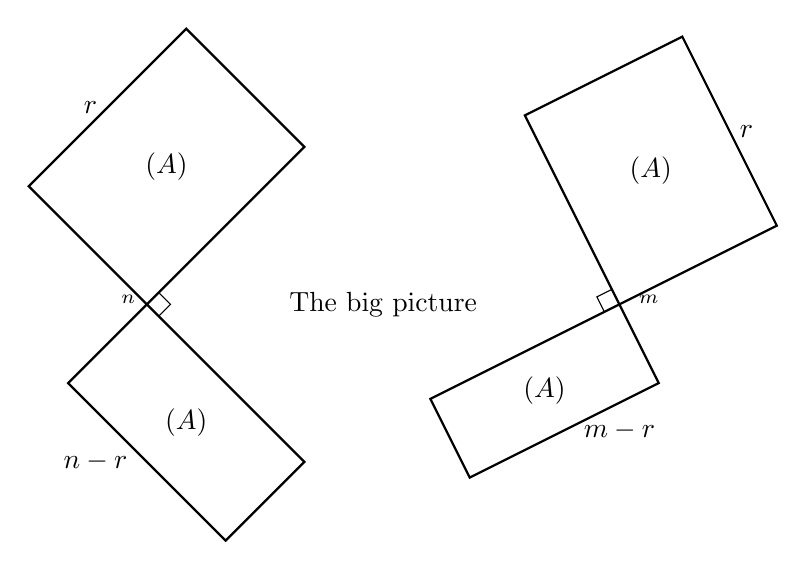
\begin{tikzpicture}
        \node at(3, 0){The big picture};
        \draw[thick](0, 0)node[left]{$\RR^n$}--(2, 2)--(.5, 3.5)--(-1.5, 1.5)node[midway, left]{$r$}--(2, -2)--(1, -3)--(-1, -1)node[midway, left]{$n-r~$}--cycle;
        \draw(.15, .15)--(.3, 0)--(.15, -.15);
        \node at(.25, 1.75){$\C(A\tp)$};
        \node at(.5, -1.5){$\N(A)$};
        \draw[thick](6, 0)node[right]{$~\RR^m$}--(8, 1)--(6.8, 3.4)node[midway, right]{$r$}--(4.8, 2.4)--(6.5, -1)--(4.1, -2.2)node[midway, right]{$~m-r$}--(3.6, -1.2)--cycle; % +6
        \draw(5.905, .19)--(5.715, .095)--(5.81, -.095); % .03√10
        \node at(6.4, 1.7){$\C(A)$};
        \node at(5.05, -1.1){$\N(A\tp)$};
    \end{tikzpicture}
    \captionof{figure}{$A$的四个子空间}
\end{center}

\subsectionstar{矩阵的秩的不等式}

% 参考:\url{https://zhuanlan.zhihu.com/p/55206421}

\begin{theorem}{}{}
	对于矩阵$A,B$有
	\begin{equation}
		\rank(A+B)\leq\rank(A)+\rank(B).
	\end{equation}
\end{theorem}
\begin{proof}
	设$\C(A),\C(B)$的一组基分别为$\{a_1,\ldots,a_{\rank(A)}\}$和$\{b_1,\ldots,b_{\rank(B)}\}$,则$A+B$中的列必然可以由$\{a_1,\ldots,a_{\rank(A)},b_1,\ldots,b_{\rank(B)}\}$的线性组合表示出,故不等式成立。
\end{proof}
\begin{theorem}{Sylvester不等式}{Sylvester inequality}
	对$n$阶方阵$A,B$有
	\begin{equation}
		\rank(AB)\geq\rank(A)+\rank(B)-n.
	\end{equation}
\end{theorem}
\begin{proof}
	注意到
	\[
		\rank(AB)+n=\rank\biggkh{\begin{bmatrix}
			I_n\\ &AB
		\end{bmatrix}}=\rank\biggkh{\begin{bmatrix}
			I_n&-B\\A
		\end{bmatrix}}\geq\rank(A)+\rank(B).\qedhere
	\]
\end{proof}

\begin{theorem}{Frobenius秩不等式}{Frobenius rank inequality}
	对于矩阵$A,B,C$,有
	\begin{equation}
		\rank(ABC)\geq\rank(AB)+\rank(BC)-\rank(B).
	\end{equation}
\end{theorem}
\begin{proof}
	注意到
	\begin{align*}
		\rank(ABC)+\rank(B)&=\rank\biggkh{\begin{bmatrix}
			B\\ &ABC
		\end{bmatrix}}\\
		&=\rank\biggkh{\begin{bmatrix}
			BC&B\\ &AB
		\end{bmatrix}}\geq\rank(AB)+\rank(BC).\qedhere
	\end{align*}
\end{proof}

